\section{Description et objectifs}
La gamification, ou ludification, est définie comme l’application d’élément issus de jeux, jeux vidéo ou autre activités ludiques à d’autre domaines. Ces éléments sont dans la majorité des cas la mise en place d’un système de score à points, d’un statut lié au niveau ou temps de jeu, de l’utilisation de tableaux de bord, de compétition (coopérative ou non) et de règles de jeu à suivre. La gamification est généralement appliquée dans le cadre du marketing afin d’augmenter l’engagement des potentiels clients envers un produit ou service.\par
Le terme et son application sont depuis quelques années devenu très à la mode dans d’autres domaines que le marketing, que ce soit lors de projets internes à une entreprise, de séminaires de cohésion d’équipe ou, dans le cadre de ce mémoire le cas qui nous intéresse, l’enseignement d’une discipline.

\section{Les mécaniques de la gamification}
Basé sur les travaux de Gabe Zihermann et d'Andrzej Marcsweski, Sarath Koppolu~\cite{gamif-thesis} définit les cinq principes de la gamification comme suit : 
\begin{enumerate}
    \item "Purpose" : la gamification doit avoir un but clair et défini dans le processus où elle est appliquée, processus dont les participants ont une connaissance suffisante pour comprendre et accepter son application
    \item "Progress" : l’accompagnement de la progression des participants, notamment via l’apprentissage de nouvelles compétences, leur affûtage ou les retours réguliers d’expérience par exemple
    \item "Proficiency" : travailler sur la motivation des participants à faire les choses parce qu’ils l’apprécient plutôt que pour simplement en obtenir quelque chose
    \item "Pride" : récompenser les participants pour leur apporter de l’estime d’eux-mêmes et maintenir leur intérêt
    \item "People" : construire le processus autour des gens au lieu de les considérer comme une simple entité du système gamifié. Construire autour des envies et besoins des gens plutôt que du système
\end{enumerate}\par

Basé sur le Framework Octalysis~\ref{fig:octalysis}, il est possible de définir et répartir divers comportements, processus et moteurs de gamification entre le "cerveau gauche" (accomplissement, possession, rareté) et le "cerveau droit" (responsabilisation, influence sociale, imprédictibilité). Il sépare également les bons comportements et influences de la gamification des néfastes, en "White hat" et "Black hat gamification". La seconde utilise la peur, l’incertitude, la perte d’opportunité pour maintenir les participants engagés, mais entraîne de nombreuses pertes pour ceux-ci à terme, que ce soit en quittant le système ou en développant des addictions diverses, là où la première encourage la créativité, récompense, encourage et aide les participants à s’améliorer afin de les maintenir engagés.

\begin{figure}
    \centering
    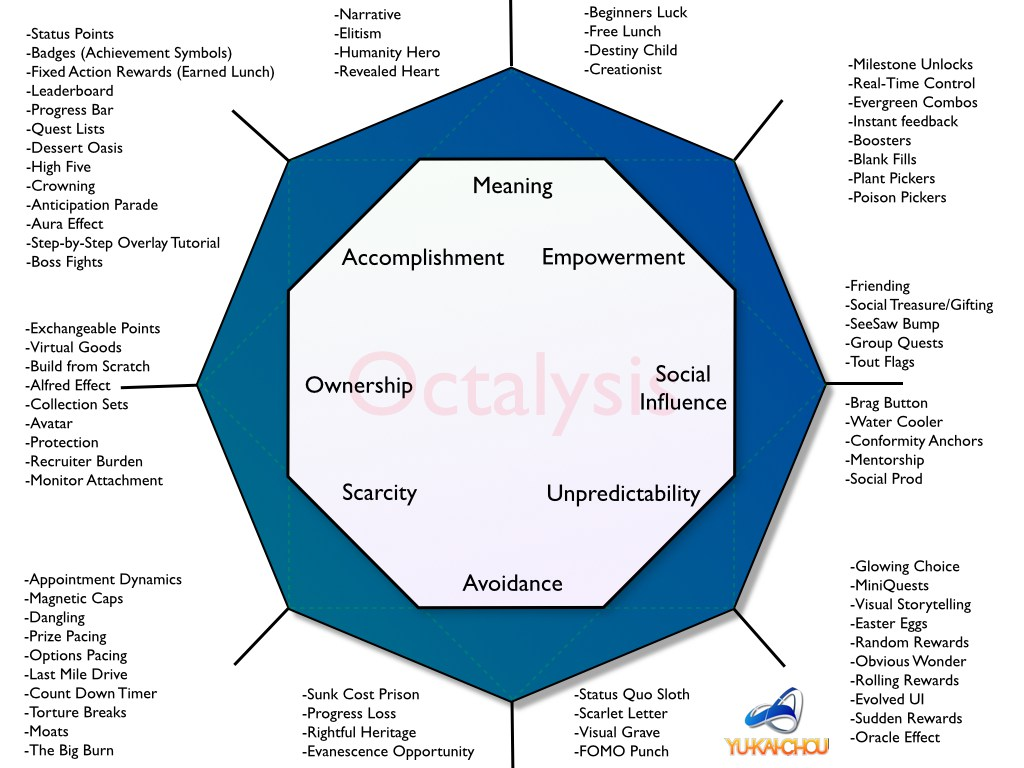
\includegraphics[width=0.9\linewidth]{Images/The-Octalysis-Framework.jpg}
    \caption{Framework Octalysis}
    \source{Yu Kai Chou, 2013}
    \label{fig:octalysis}
\end{figure}

\section{Types de participants}
En se basant sur la taxinomie de Richard Bartle et les travaux de Alexandra Iosup et Dick Epema~\cite{gamif-educ, gamif-taxonomy}, on peut identifier quatre types d'étudiants dans le cadre d'un enseignement gamifié~\ref{fig:bartle} :
\begin{itemize}
    \item Les "Explorers" sont ceux qui aiment comprendre et découvrir le monde, les curieux. Ils sont à la fois intéressés par la qualité et la quantité des enseignements
    \item Les "Achievers" sont ceux qui aiment réussir les challenges auxquels ils sont confrontés, les ambitieux qui en plus de valider le cursus le font avec les meilleurs résultats
    \item Les "Socialisers" sont ceux qui participent principalement parce que d’autres personnes comme eux le font également ; réussir le cursus les intéresse surtout s’ils maintiennent leur cercle social
    \item Les "Winners", ou "Killers" dans la taxinomie originale, sont ceux qui veulent réussir au dépend des autres participants. Pour eux, un challenge n’a de sens que s’il n’y a qu’un seul gagnant, si possible eux. Cette tendance à la compétitivité peut être autodestructrice, et mener à l’ennui, au burn-out, voire à la dépression
\end{itemize}

\begin{figure}
    \centering
    
\includegraphics[width=0.5\linewidth]{Images/Character_theory_chart.png}
    \caption{Catégories de joueurs}
  
    \source{Richard Bartle, 1996}
    \label{fig:bartle}
\end{figure}


\section{Différence avec les "Jeux sérieux"}
Un jeu sérieux, de l'anglais "serious game", est une activité mêlant une intention pédagogique ou informative ("sérieuse") avec des ressorts ludique, ici le jeu. On peut résumer un jeu sérieux à un jeu de société, de rôle ou vidéo qui s'éloigne du seul but de divertissement ou amusement. \par
La vocation d'un jeu sérieux est de rendre sa composante sérieuse attrayante via son côté ludique et interactif. Là où la gamification vise à introduire à un enseignement ou projet des mécaniques et aspects issus de jeux pour en augmenter l'engagement et l'efficacité, les jeux sérieux sont d'avantage des outils complémentaires à l'enseignement. Ils permettent d'apprendre ou de consolider des connaissances via le jeu, là où la gamification est une forme d'apprentissage et de réalisation à part entière.